\subsection{MEX 2-3: Effect of compressibility on pressure driven percolation}

Participating institutions of MEX 2-3 (see section \ref{sec:mex04}): CAU, IfG, UFZ

\begin{table}[ht!]
\caption{MEX 2-3: Data overview}
\label{tab:dms-mex23-overview}
\small
\begin{tabular}{l|l|l|l|L{4.7cm}|l}
\hline
\rowcolor{cyan}
Type & Spec. & Owner & Access     & Comment                       & Stat \\ 
\hline 
EXP  & LIT   & \cite{Kamlot2009} & Restricted & Literature available online & \cellcolor{green} \\
\hline \hline
MOD  & LEM   & CAU   & License    & Executable MATLAB P-file      & \cellcolor{yellow} \\
     &       &       & Free       & I/O available                 & \cellcolor{yellow} \\
\hline
MOD  & DEM   & IfG   & License    & Commercial software           & \cellcolor{green} \\
     &       &       & Free       & I/O available                 & \cellcolor{yellow} \\
\hline
MOD  & FEM   & UFZ   & Open source & via OpenGeoSys portal        & \cellcolor{yellow} \\
     & VFP   &       & Free        & I/O available                & \cellcolor{green} \\
%
\hline
\end{tabular}
\end{table}
\normalsize

\subsubsection*{CAU Kiel}

The required LEM code and the input variables for simulating the effect of compressibility are uploaded to the IfG (Kiel) NextCloud server. The data is accessible through the following link:\\
\url{https://nextcloud.ifg.uni-kiel.de/index.php/s/6Mfg3P4PyKNN6By}

The uploaded protected MATLAB file in a *.p format requires a MATLAB version with a built-in Voronoi Tessellation and Delaunay Triangulation functions. The input variables are prepared in two different files for the simulation of the pressure drop in gas and brine reservoirs. Fig. \ref{fig:Amir_ME4_Pressure_Data} shows the differences between the pressure drop in gas and brine reservoirs.

\begin{figure}[!ht]
\centering
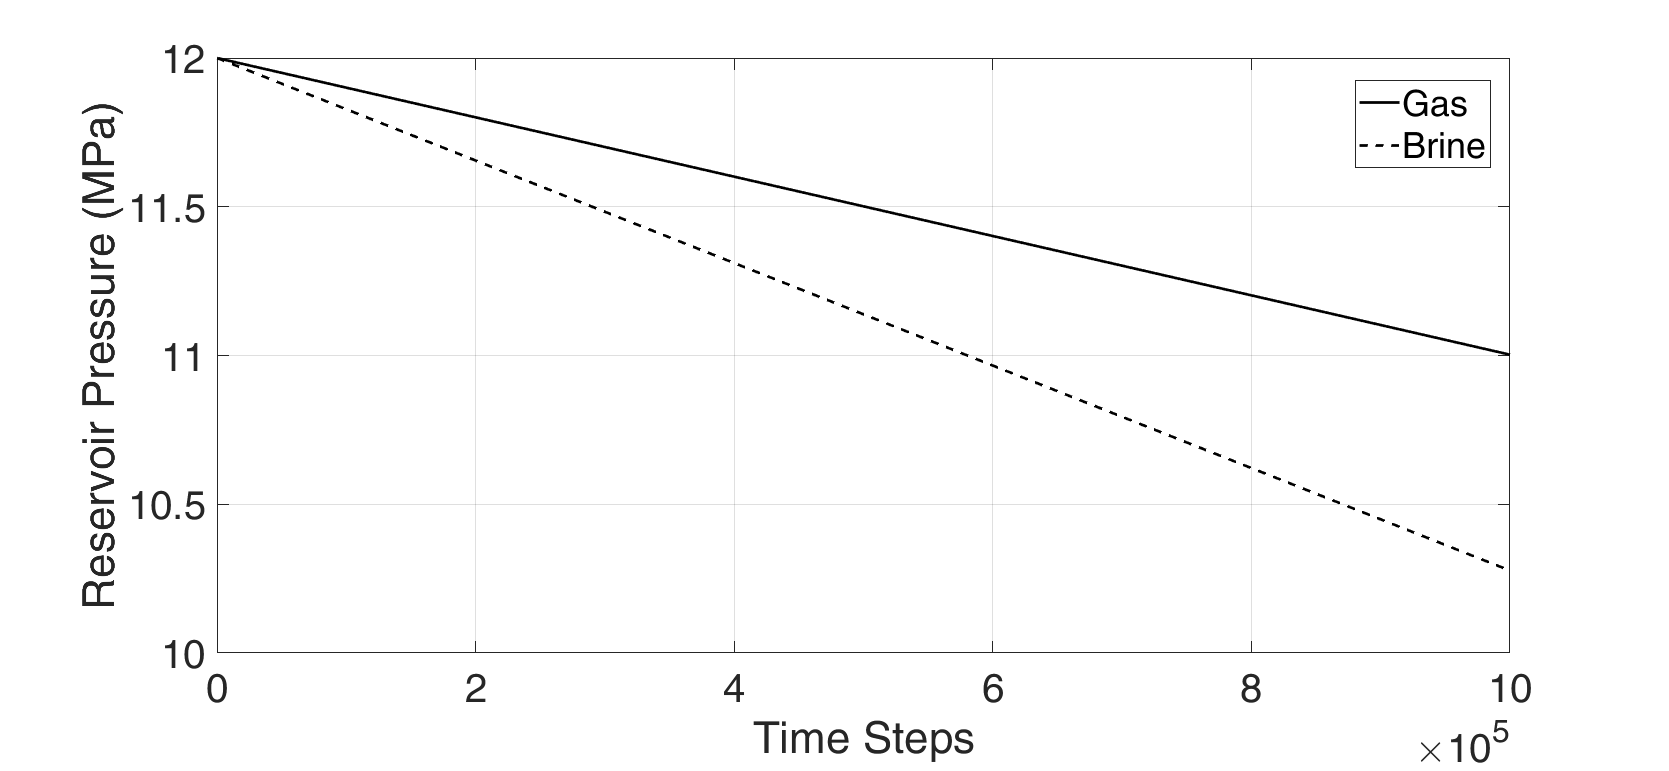
\includegraphics[width=0.6\textwidth]{figures/Amir_ME4_Pressure_Data.png}
\caption{The comparison between the pressure drop in gas and brine reservoirs}
\label{fig:Amir_ME4_Pressure_Data}
\end{figure}

%\subsubsection*{IfG}
%\subsubsection*{UFZ}

\clearpage
%---------------------------------------------------------
\subsubsection*{Meta Data Overview (according to Dublin Core)}
%---------------------------------------------------------

\begin{table}[!ht]
\caption{MEX 2-3: Meta Data according to Dublin Core}
\label{tab:dms-mex23}
\small
\begin{tabular}{R{3.5cm}|L{7.5cm}}
\hline
%
Data label & GeomInt, MEX 2-3, CAU, effect of compressibility, salt\\
URL (Numerics) & \url{https://nextcloud.ifg.uni-kiel.de/index.php/s/6Mfg3P4PyKNN6By} \\
Subject  &  Effect of compressibility (Saltstone)\\
Type of data  & Executable MATLAB P-file, Input parameters\\
Data quality  &  Quality assured data \\
Status of data  &  Unprocessed data\\
Data format  & txt, MATLAB executable P-file\\
Creators  &  Kiel University, Institute of Geomechanics and Geotechnics, Ludewig-Meyn-Stra\ss e 10, 24118, Kiel\\
Source/Origin & In-house code \\
Publisher  &  Kiel University, Institute of Geomechanics and Geotechnics, Ludewig-Meyn-Stra\ss e 10, 24118, Kiel \\
Rights holders &  Kiel University, Institute of Geomechanics and Geotechnics, Ludewig-Meyn-Stra\ss e 10, 24118, Kiel \\
Contributors &   Kiel University, Institute of Geomechanics and Geotechnics: Amir Shoarian Sattari, Frank Wuttke \\
Time/period of creation &  2019-2020\\
Language of the content &  English\\
Update policy &  Stored data is final\\
Access permissions & Full access\\
%
\hline
\end{tabular}
\end{table}


